\chapter{esaについて}

esaではいつかのアップデートで、直接Githubに記事を保存ができるようになりました。
2016年のアップデートらしいですね。
細かい設定などは下の記事でご確認ください。

\url{https://docs.esa.io/posts/176}

では、とりあえず設定をしていきましょう。

\section{設定}

  まずは、esaの設定をしましょう。
  
  \begin{figure}[H]
    \centering
    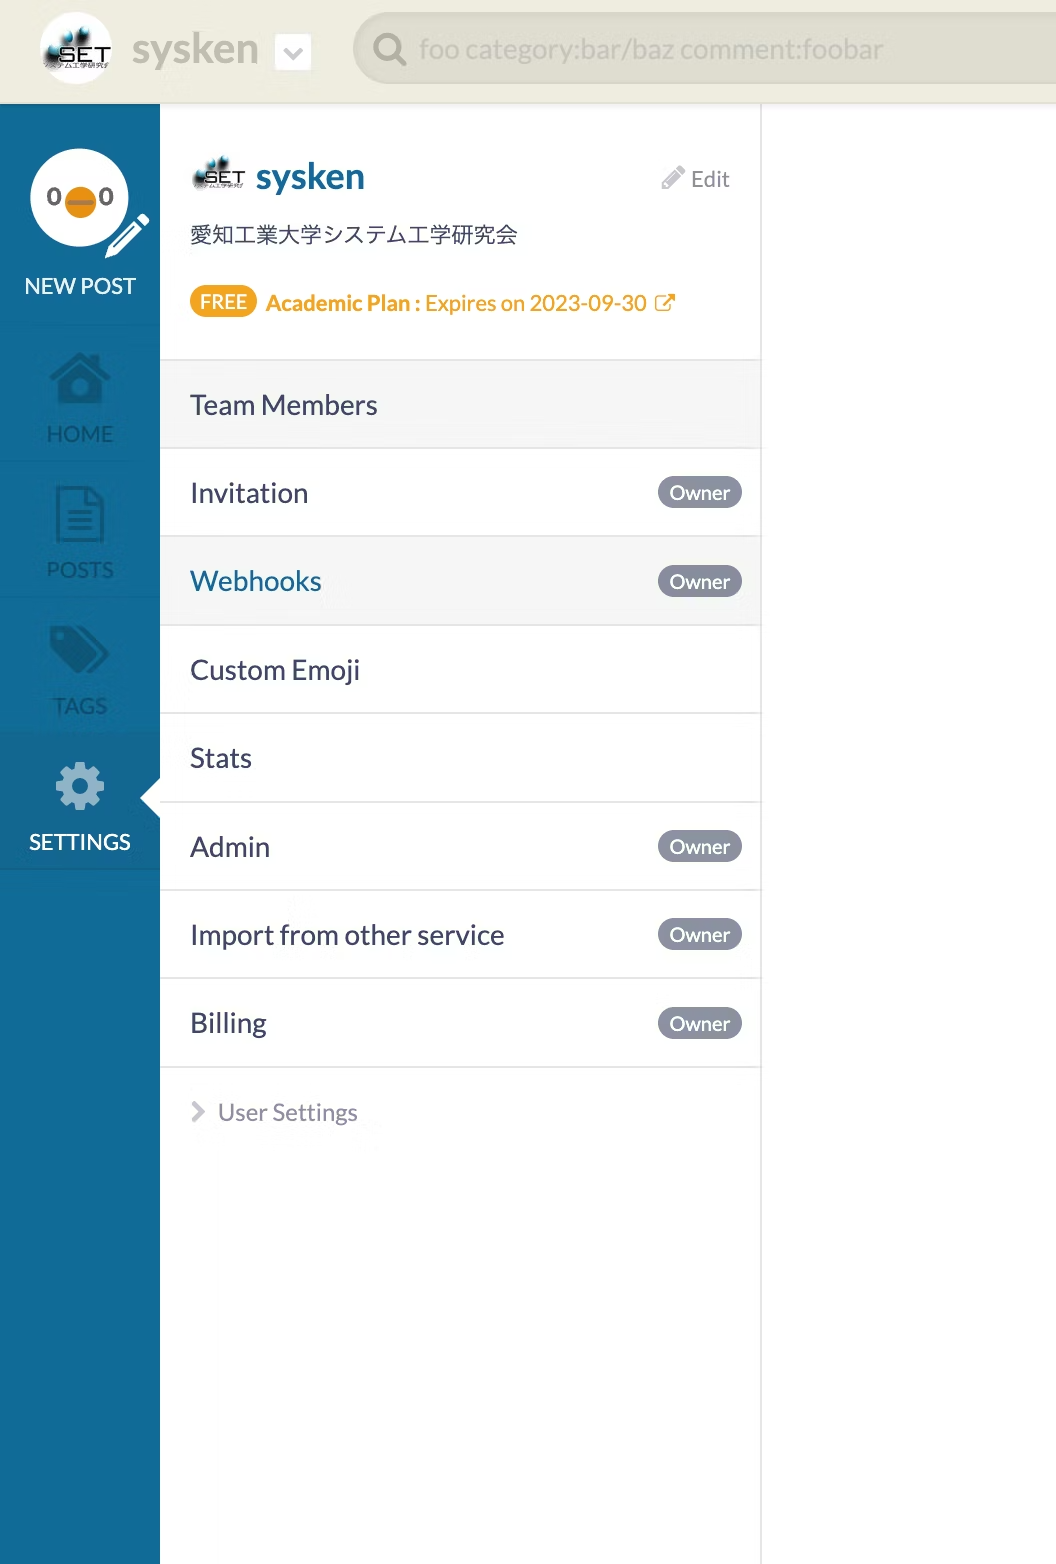
\includegraphics[width=8cm]{./image/02-chap7/esa-setting.png}
    \caption{esaの設定画面}
    \label{chap7-esa-setting-image}
  \end{figure}

  setting -> Webhooksを選択します。

  addを選択して、Github(β)を選択します。 

  \begin{figure}[H]
    \centering
    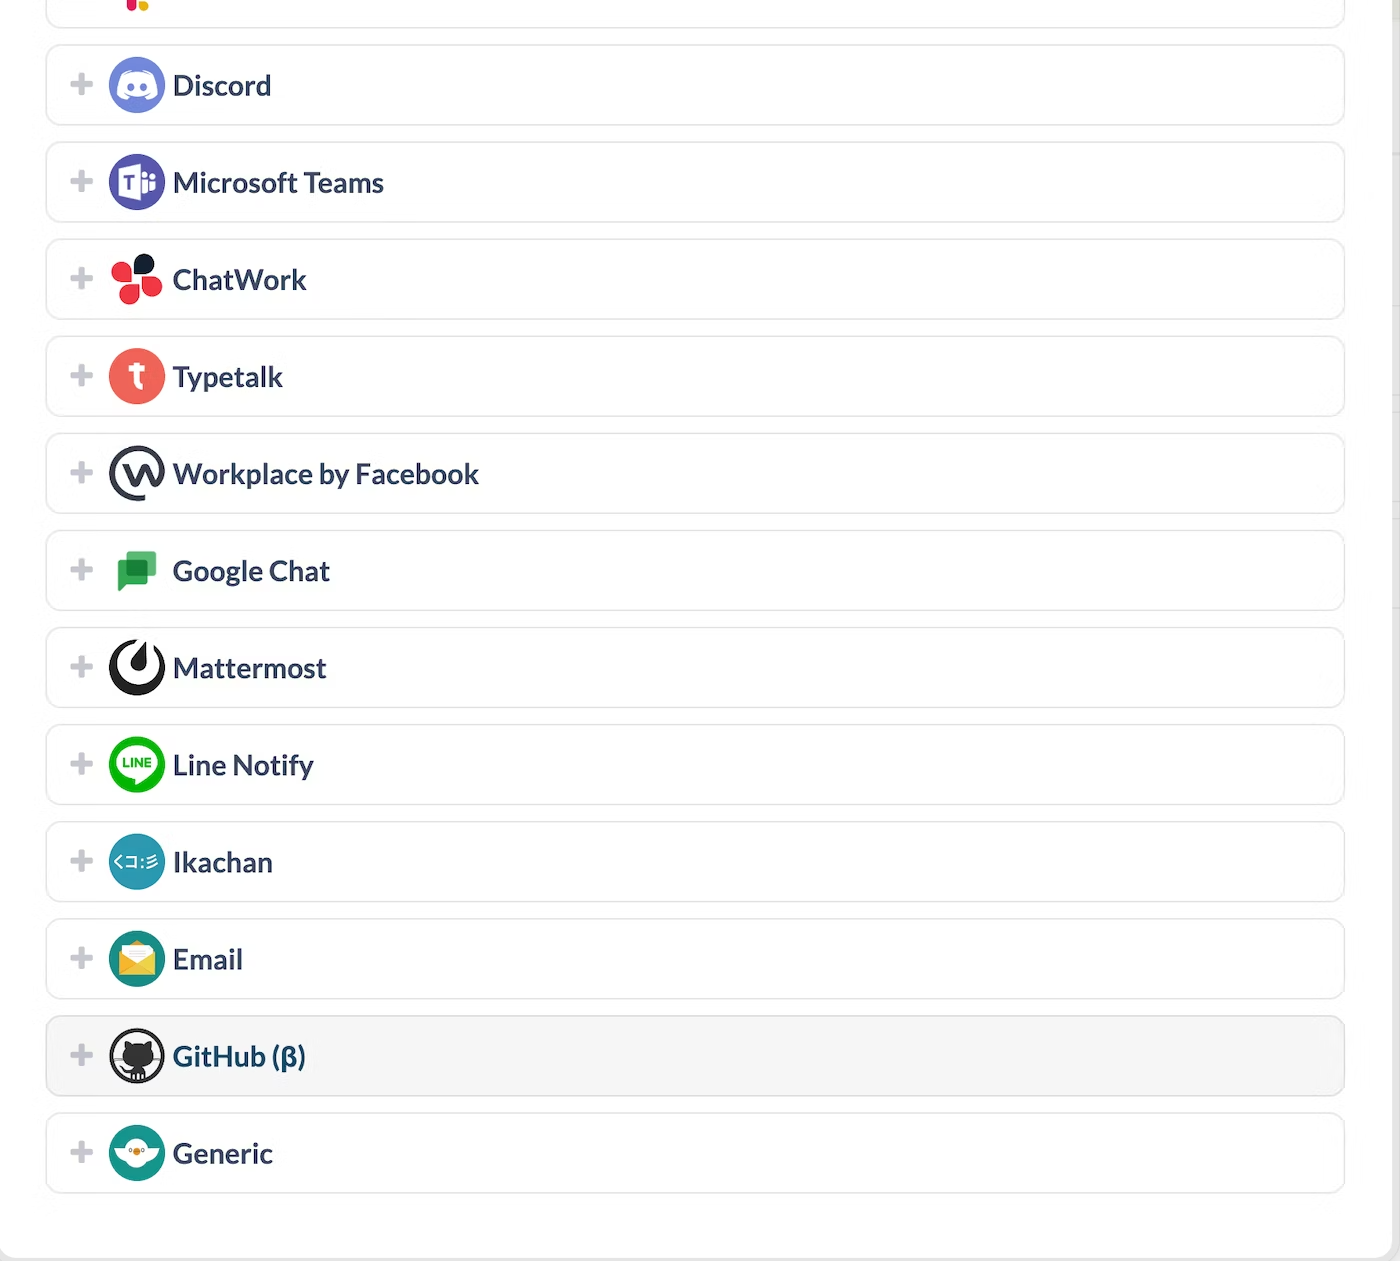
\includegraphics[width=8cm]{./image/02-chap7/esa-setting-list.png}
    \caption{esaの設定画面 API連携の部分 }
    \label{chap7-esa-setting-list-image}
  \end{figure}

  あとは、様々な設定を行って、保存をします。

  esa root category
  ここで、Webページに更新されて欲しい記事のディレクトリを選択することもできるので設定してみてください。
  output directory
  出力の場所はhugoの関係で指定しないといけないので、/content/post/と設定しましょう。

  \begin{figure}[H]
    \centering
    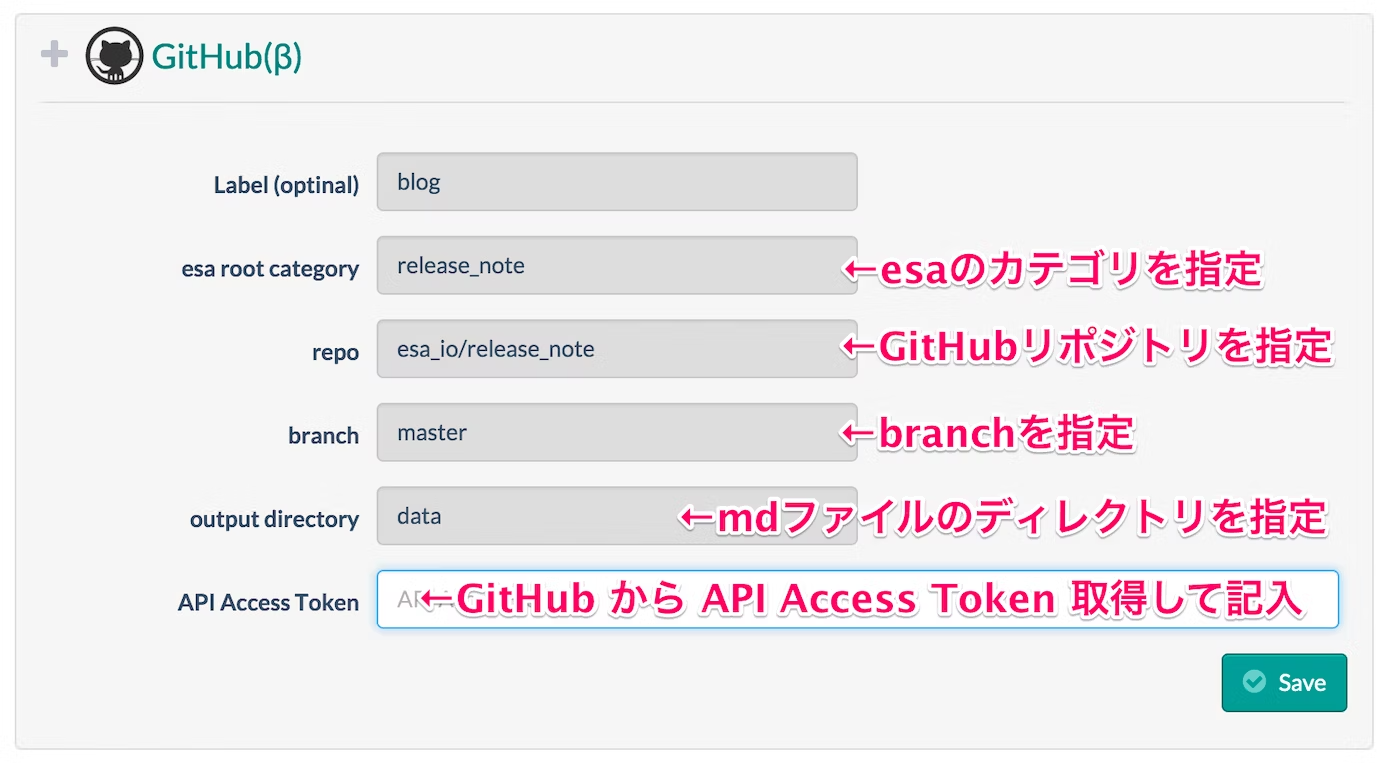
\includegraphics[width=8cm]{./image/02-chap7/github-setting.png}
    \caption{esaの設定画面 Githubの設定 }
    \label{chap7-github-setting-image}
  \end{figure}

  \begin{figure}[H]
    \centering
    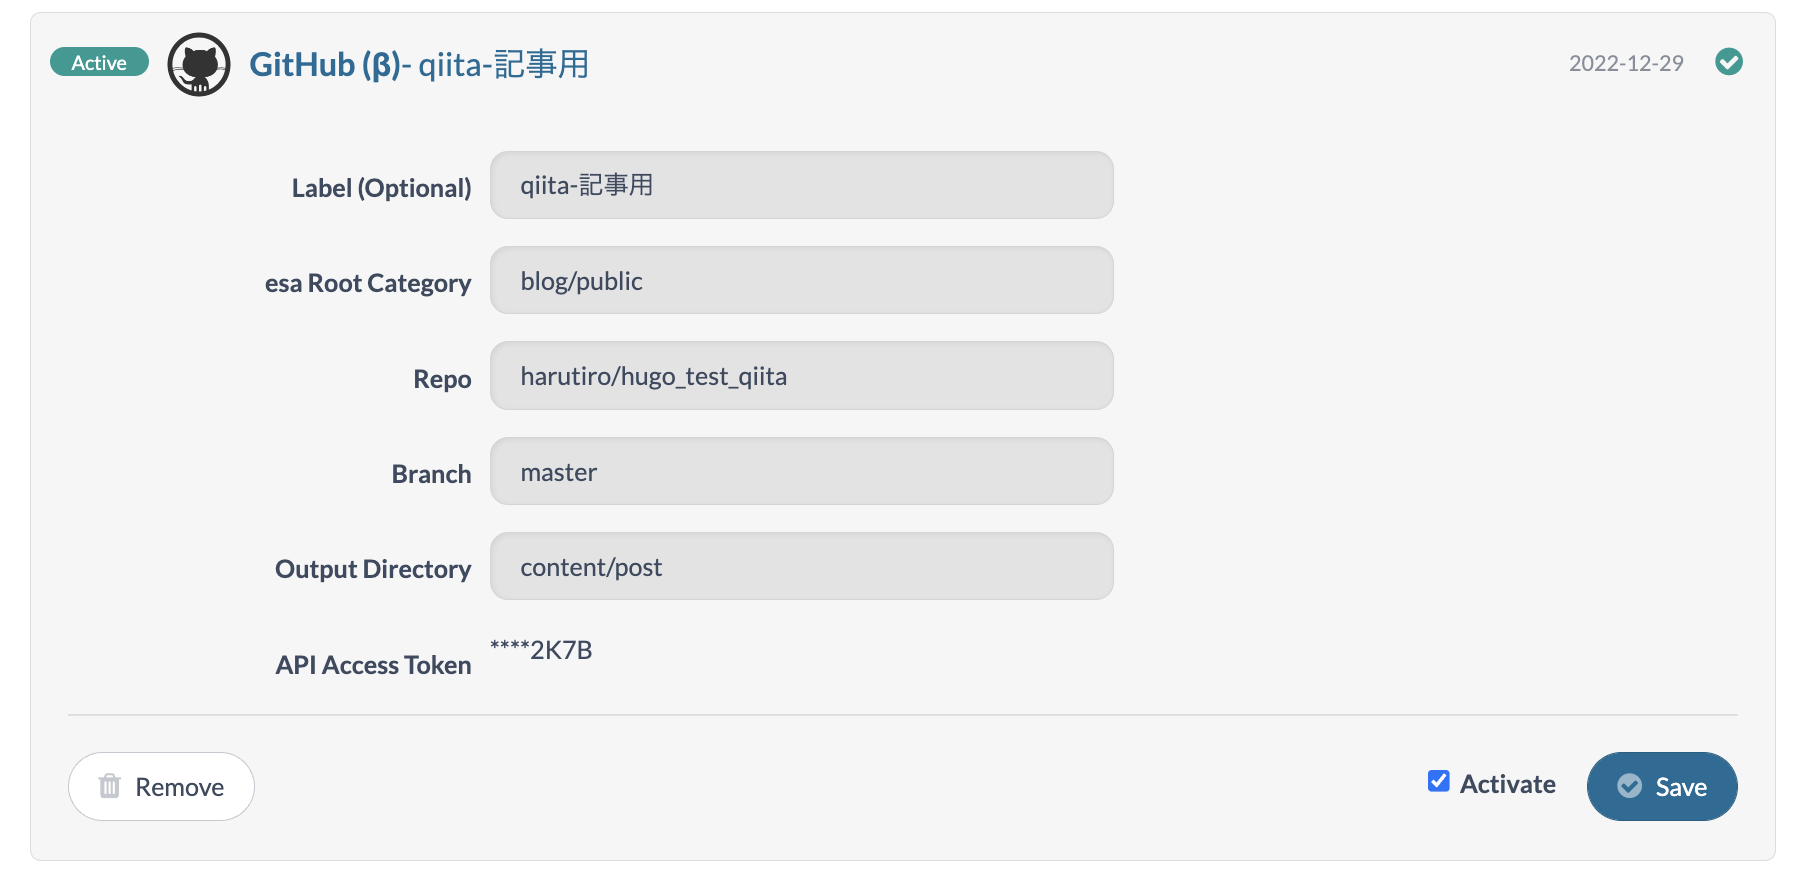
\includegraphics[width=8cm]{./image/02-chap7/github-setting-writed.png}
    \caption{esaの設定画面 Githubの設定 実際の設定項目 }
    \label{chap7-github-setting-writed-image}
  \end{figure}

  これで記事が更新(新規)で作られたら、Githubのレポジトリの更新されました。

  では、実際にesaが更新されたらpostに新しいファイルが追加されるか確認してみましょう。

  こういったファイルを投稿してみました。

  \begin{figure}[H]
    \centering
    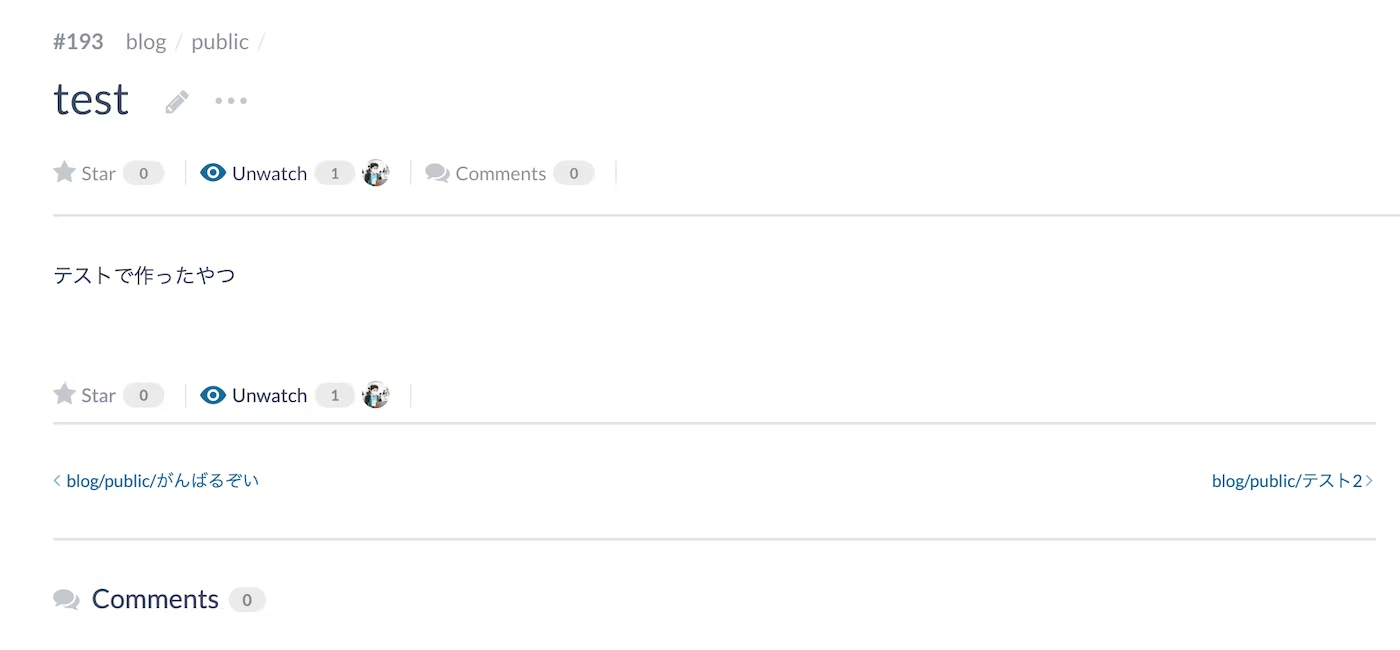
\includegraphics[width=8cm]{./image/02-chap7/esa-posted.png}
    \caption{esaに投稿した記事 }
    \label{chap7-esa-posted-image}
  \end{figure}

  ファイルが新しく追加されてますね。

  \begin{figure}[H]
    \centering
    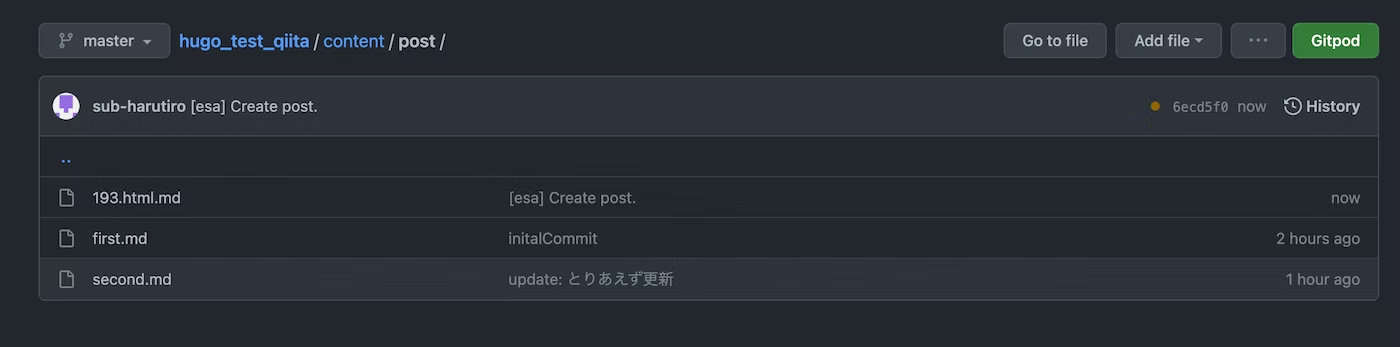
\includegraphics[width=8cm]{./image/02-chap7/github-upload-image.png}
    \caption{Githubに記事が追加された }
    \label{chap7-github-upload-image-image}
  \end{figure}

  しかし、このままだとWebページは更新されていません。
  それはhugoを用いて静的なファイルを生成していないためです。

  では次の章ではGithubActionsを用いてhugoを実行するプログラムを書いていきましょう。




  
  
  